\section{Obstacle Avoidance: Benchmark}
\label{sec:avoidance}
Obstacle avoidance is vital for drone flights at low altitude (up to a
few hundred feet) in urban or forested settings. Otherwise, being restricted to only high altitude flight impairs visual detections and hides many details.  The most dangerous obstacles are
typically trees, lightposts, and telephone poles, which can easily
reach altitudes usually used by drones. Being  relatively thin,
they are difficult to detect from afar.  

Efficient avoidance of such obstacles is a challenge.  Since drone
flight is limited by battery life (typically on the order of 30-50
minutes), bypassing obstacles without wasting too much flight time is
important. If flight is too slow or avoidance maneuvers are too
convoluted, mission performance will be impaired.  At the same time,
reckless flight could be catastrophic.  Striking the right balance
between safety and speed for the given flight conditions is essential.
Since effective but rapid avoidance of obstacles is a valuable
capability in a drone, this task is a good candidate for an agility
benchmark.

\subsection{Benchmark Requirements}
\label{sec:avoidance-requirements}

A good benchmark for this task should capture the essential difficulty
of obstacle avoidance.  It should be parameterized, so that it is easy to
vary the difficulty of the benchmark.  The benchmark should only use
standardized, off-the-shelf components that can be easily purchased or
fabricated.  There should be no ambiguity in the experimental setup or
interpretation of results, thereby simplifying independent attempts to
reproduce published experimental results.
\S\ref{sec:avoidance-description} presents my candidate benchmark
that meets these requirements.

\subsection{Benchmark Description}
\label{sec:avoidance-description}

\begin{figure}
    \centering
    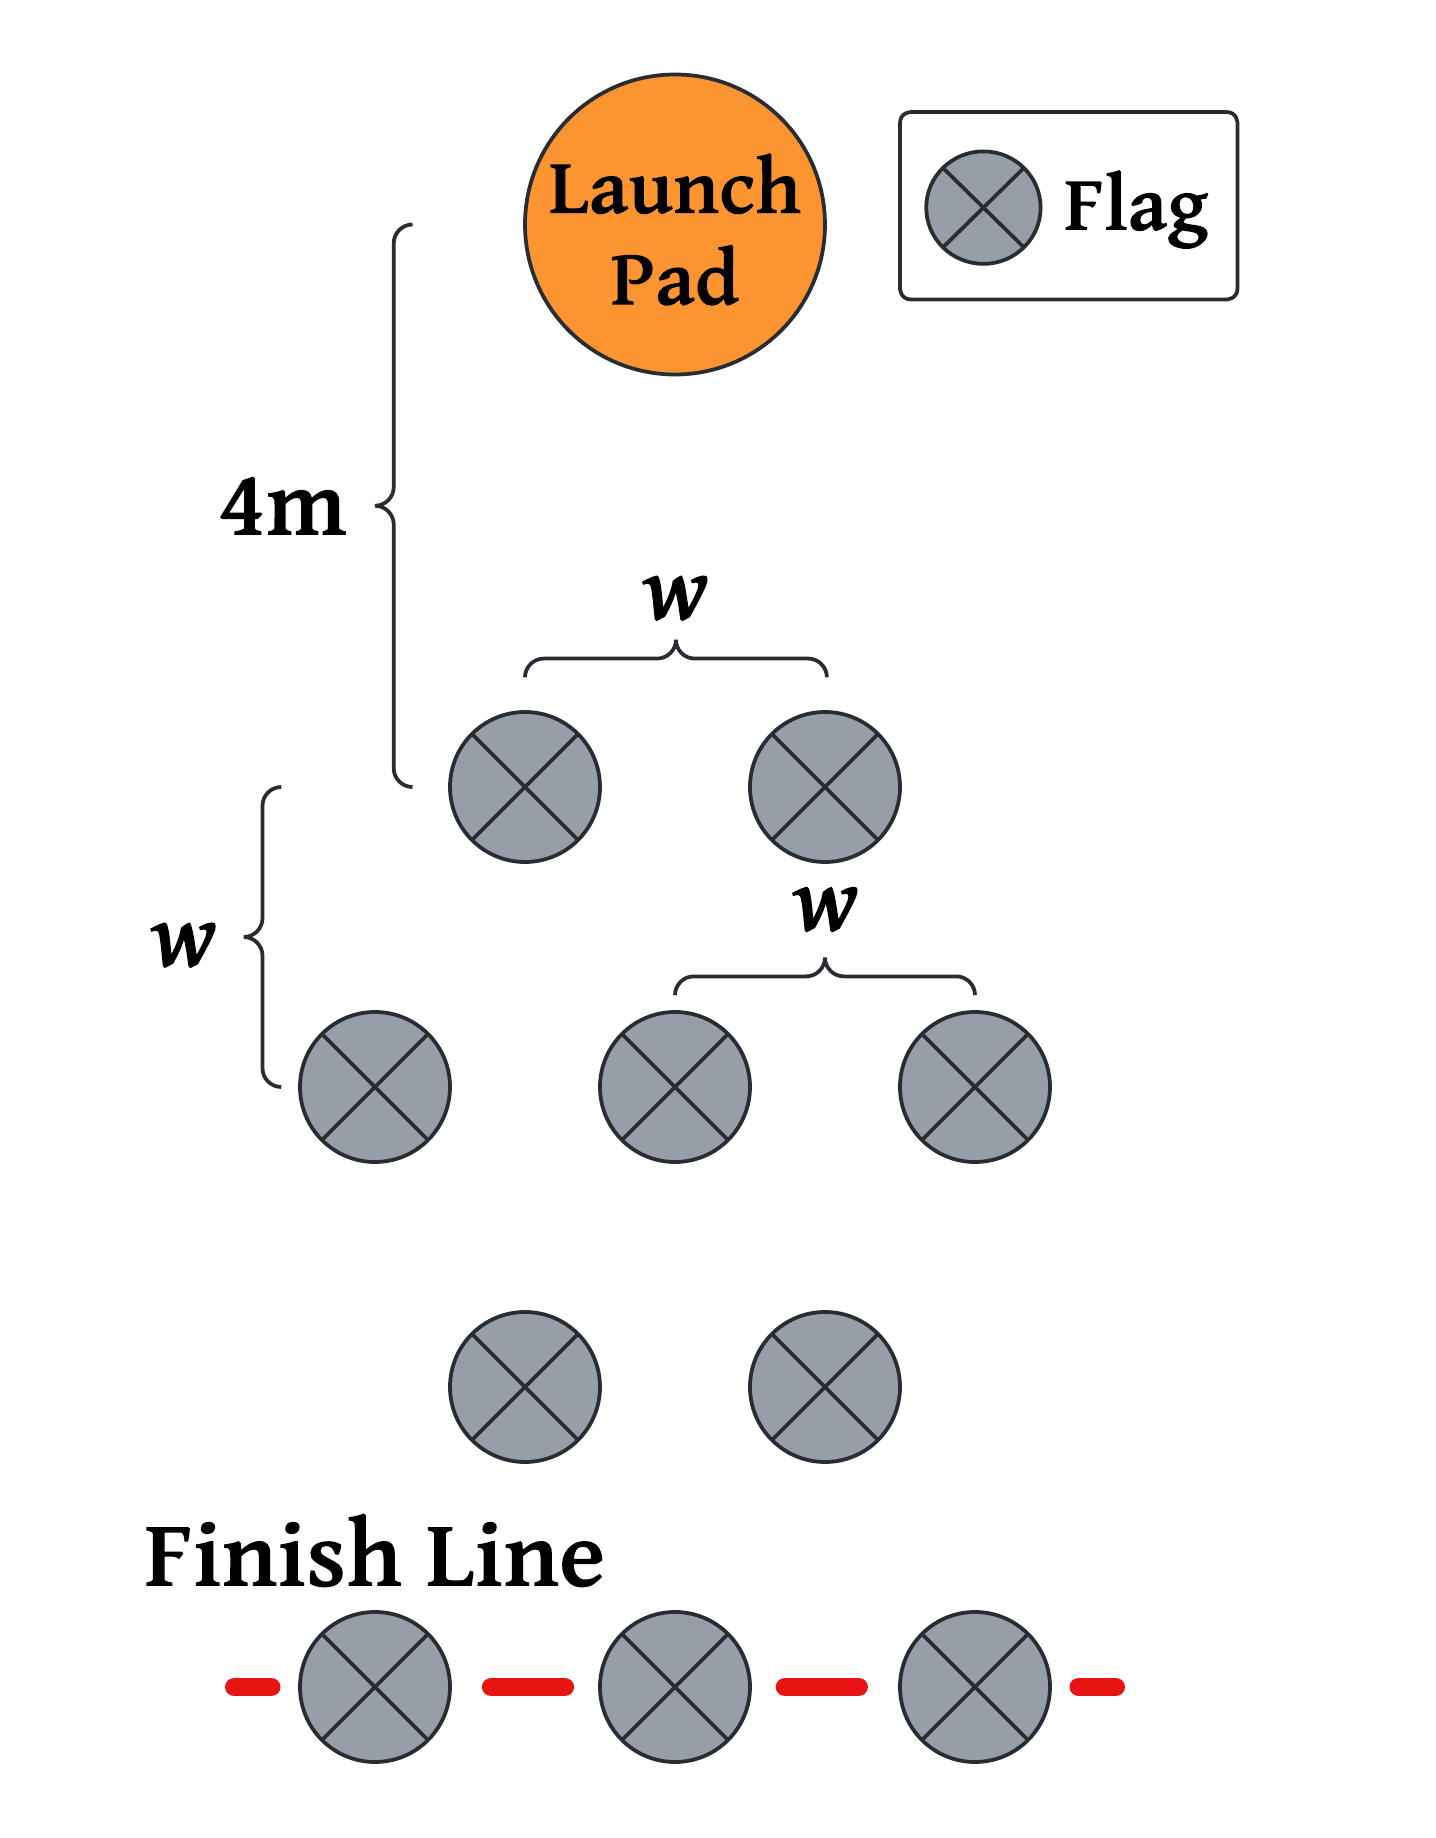
\includegraphics[trim=-4cm 0 0 0, width=0.5\linewidth]{chapter6/FIGS/fig-obstacle-course.png}
    \caption{Obstacle Course Layout}
    \label{fig:obstacle-course}
\end{figure}

To emulate tall and skinny obstacles such as lightposts, I use 1.8~m
long drone racing flags.  The flags are
arranged in a precisely-defined slalom
pattern~(Figure~\ref{fig:obstacle-course}), that forces a drone to
sequentially evade several obstacles.  The difficulty of the course is
controlled by a spacing parameter, $w$, that determines the separation
of the flags along both the azimuth and range axes.  A smaller value
of $w$ defines a more difficult course because of higher density of
obstacles in both directions.  All my experiments were conducted with
4 tiers of obstacles.  Adding more tiers to make the obstacle course
longer, while preserving obstacle spacing, would add further
difficulty to the course.  The drone's goal is to navigate the course
as fast as possible, without touching the flags or striking a
flagpole.  The metric of interest is the transit time through the
course.

To execute this benchmark, the obstacle course is set up as in
Figure~\ref{fig:obstacle-course}.  The drone is placed on a pad that
is centered 4~m in front of the leading line of flags.  A human
spotter stands a safe distance behind the drone, and a human
timekeeper is positioned along the finish line.  The remote
pilot-in-command (RPIC) continuously monitors the video stream from
the drone, and stands ready to wrest back manual control if the
drone's autonomous flight software appears to be getting it into
trouble.  Such a manually aborted flight is scored as ``Did Not
Finish~(DNF).''  A flight in which the drone touches a flag
or pole is also scored as DNF.

The drone takes off and then hovers at an altitude of 1~m.  It
is then directed to autonomously move to a destination beyond the
obstacle course. When forward motion begins, the spotter visually
signals the timekeeper to start a stopwatch. The spotter then follows
the drone through the course, warning the RPIC of imminent collision,
if any.  Such a warning aborts the experiment without damage to the
drone.  On a successful flight, timing is stopped as soon as the
trailing end of the drone crosses the finish line.  We deem an
obstacle spacing, $w,$ as viable if the drone successfully flies
through the course on at least 80\% of its attempts.  The average time
of these successful flights at the smallest viable $w$ is the figure
of merit. For small values of $w$, a more agile drone can fly more
aggressively and therefore requires less time to complete the benchmark.
However, at higher values of $w$, agility may not be important because
the obstacle course easier.

\begin{table}
\small
	\centering
        \begin{tabular}{|c|c|c|}
		\hline
		\textbf{Model} & \textbf{Latency (ms)} & \textbf{Throughput (fps)} \\
		\hline
		MiDaS Small & 61 & 10 \\
		DPT Hybrid & 105 & 8 \\
		DPT Large & 132 & 7 \\
		\hline
	\end{tabular}
\begin{captext}
\centering
    \\[0.1cm]
  \small These numbers were obtained on the cloudlet described in
  \S\ref{sec:cloudlet}
\end{captext}
\caption{Inference Speeds of MiDaS DNN Models}
\label{tab:midas-model-stats}
\end{table}

\subsection{Benchmark Scoring}
\label{sec:avoidance-scoring}

The average time, $t_{\text{avg}}$, for multiple experimental runs at
the lowest viable $w$ is a raw measure of agility.  However, this needs
to be normalized with respect to attributes other than agility.
For example, a drone whose top speed is low relative to other drones
may be penalized unfairly when measuring agility.  A low value of
$t_{\text{avg}}$ in that case is not due to a poor \ooda~loop, but
simply reflects the ``brute force'' attribute of top speed.  The
normalization is performed by removing flags from the course and
conducting a control experiment at top speed.  We denote the average
time for multiple runs of the control experiment as $t_{\text{min}}$.
The score, $S_w$, is then given by:
\begin{equation}
	S_w = \frac{t_{\text{min}}}{t_{\text{avg}}}\label{eq:1}
\end{equation}
Scores for this benchmark thus lie in the interval $0 < S_w \leq 1$
where $S_w = 1$ is the best possible score. A score of 0 is awarded
when a drone cannot achieve a successful completion rate of at least
80\% of the runs for the given value of $w$.

\subsection{Depth Sensing}
\label{sec:midas}

I use the same MiDaS-based avoidance algorithm described in Section~\ref{sec:midas-algorithm}. For this task, the \ooda~loop determines the speed and accuracy with which the drone can acquire fresh frames, execute the MiDaS algorithm on them, calculate new headings for safety, and perform actuations towards those headings.  In the context of \S\ref{sec:cloudlet}, MiDaS represents Stage-2 of cloudlet processing.  Stage-3 is the processing of MiDaS output to determine a new heading, and generating the actuation command. Figure~\ref{fig:midas-sample-course} shows the algorithm running on a setup benchmark course.

\begin{figure}
	\begin{minipage}{0.495\linewidth}
		\centering
		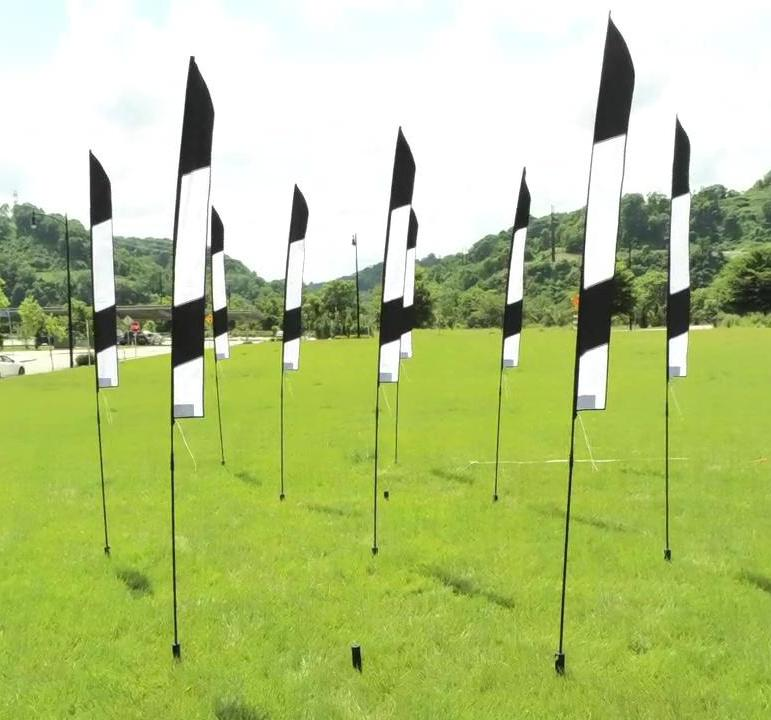
\includegraphics[width=0.8\linewidth]{chapter6/FIGS/fig-obstacle-course-drone-pov.jpg}\\
		{(a) Raw Input}\\
	\end{minipage}
	\begin{minipage}{0.495\linewidth}
		\centering
		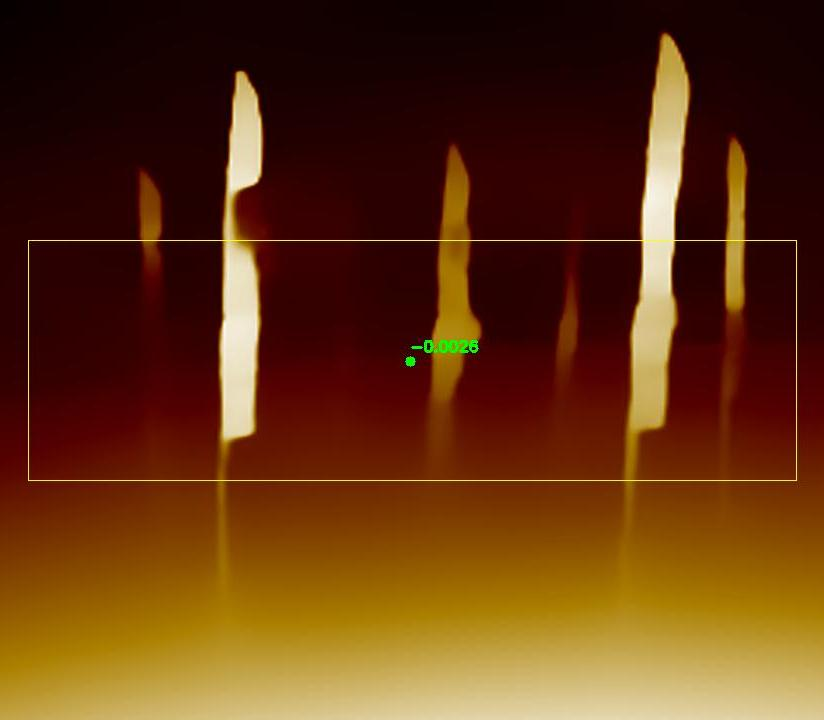
\includegraphics[width=0.8\linewidth]{chapter6/FIGS/fig-obstacle-course-midas.jpg}\\
		{(b) Output of MiDaS}\\
	\end{minipage}
\caption{MiDaS Running on the Benchmark Course}
\label{fig:midas-sample-course}
\end{figure}

I explore three DNN variants of MiDaS that vary in accuracy and speed:
{\em MiDaS Small,} {\em DPT Hybrid}, and {\em DPT Large}.  MiDaS Small
prioritizes throughput and inference latency at the cost of lower
accuracy. DPT Hybrid strikes a compromise between speed and accuracy.
DPT Large prioritizes accuracy above all else.  Figure
\ref{tab:midas-model-stats} shows the inference latency and throughput
of these three models on my cloudlet.  I explore the use of all three in my experiments.


\section{Obstacle Avoidance: Results}
\label{sec:avoidance-results}
The most basic questions in my evaluation are as follows:
\begin{itemize}
\item{\em What is the smallest value of $w$ for which the drone can
    successfully complete the benchmark?}

\item{\em At that $w$, how fast is benchmark completion?}

\item{\em As $w$ is increased, how much faster is the drone able to
    complete the benchmark?}
\end{itemize}

Initial experiments showed that 2~m is the smallest value of $w$
that meets my criterion for successful benchmark completion (i.e., at
least 80\% of the flights are successful).  Using the scoring
criterion described in \S\ref{sec:avoidance-scoring},
Figure~\ref{fig:avoid-best} shows how well the drone
 did for $w$ set
to 2~m, 2.5~m, and 3.0~m.  The results shown are the mean of 5 runs of
each experiment.  For each value of $w$, the drone results were
obtained with the choice of MiDaS model that gave the best results.
These choices were DPT Large for $w = $2~m, and MiDaS Small for $w =
2.5$~m and $w = 3$~m.  The scores of 0.13 to 0.2 show that the drone
suffers almost an order of magnitude slowdown when avoiding obstacles,
relative to its unimpeded traversal of the course.  This is the price
of having to execute the \ooda~loop shown in
Figure~\ref{fig:ooda-scaling}, with the additional Stage-2 and Stage-3
processing for depth estimation described in \S\ref{sec:midas}.  As
$w$ is increased from 2~m to 3~m, Figure~\ref{fig:avoid-best} shows
the score improving from 0.13 to 0.2.  This confirms my expectation
that less challenging courses are faster to traverse.

Since humans are the standard against which AI systems are measured,
I ask how a human pilot does under identical conditions. To
explore this, an experienced RPIC with several dozen hours of flight
time on the Parrot ANAFI platform manually executed the benchmark for
the same values of $w$. The \ooda~loop is now cyber-human: the RPIC uses the drone's live video stream to manually fly it.  Of course, a human also
has foreknowledge of the obstacle course and can subconsciously
leverage that knowledge in planning the drone's flight.  In contrast,
the autonomous drone is purely reactive --- what it sees right now is
all that it knows.

Figure~\ref{fig:avoid-human} presents my results.  Relative to
unimpeded traversal of the course, the scores of 0.76 to 0.46 show
that even the RPIC suffers a slowdown.  However, the slowdown is much
smaller than that suffered by the autonomous drone in
Figure~\ref{fig:avoid-best}.  Since the drone hardware and wireless
network are identical in the two sets of experiments, the difference
is due to the superior \ooda~loop of the human.  There is
clearly ample headroom for improvement of the drone's \ooda~loop.

\begin{figure}
\centering
\begin{minipage}{0.45\linewidth}
\centering
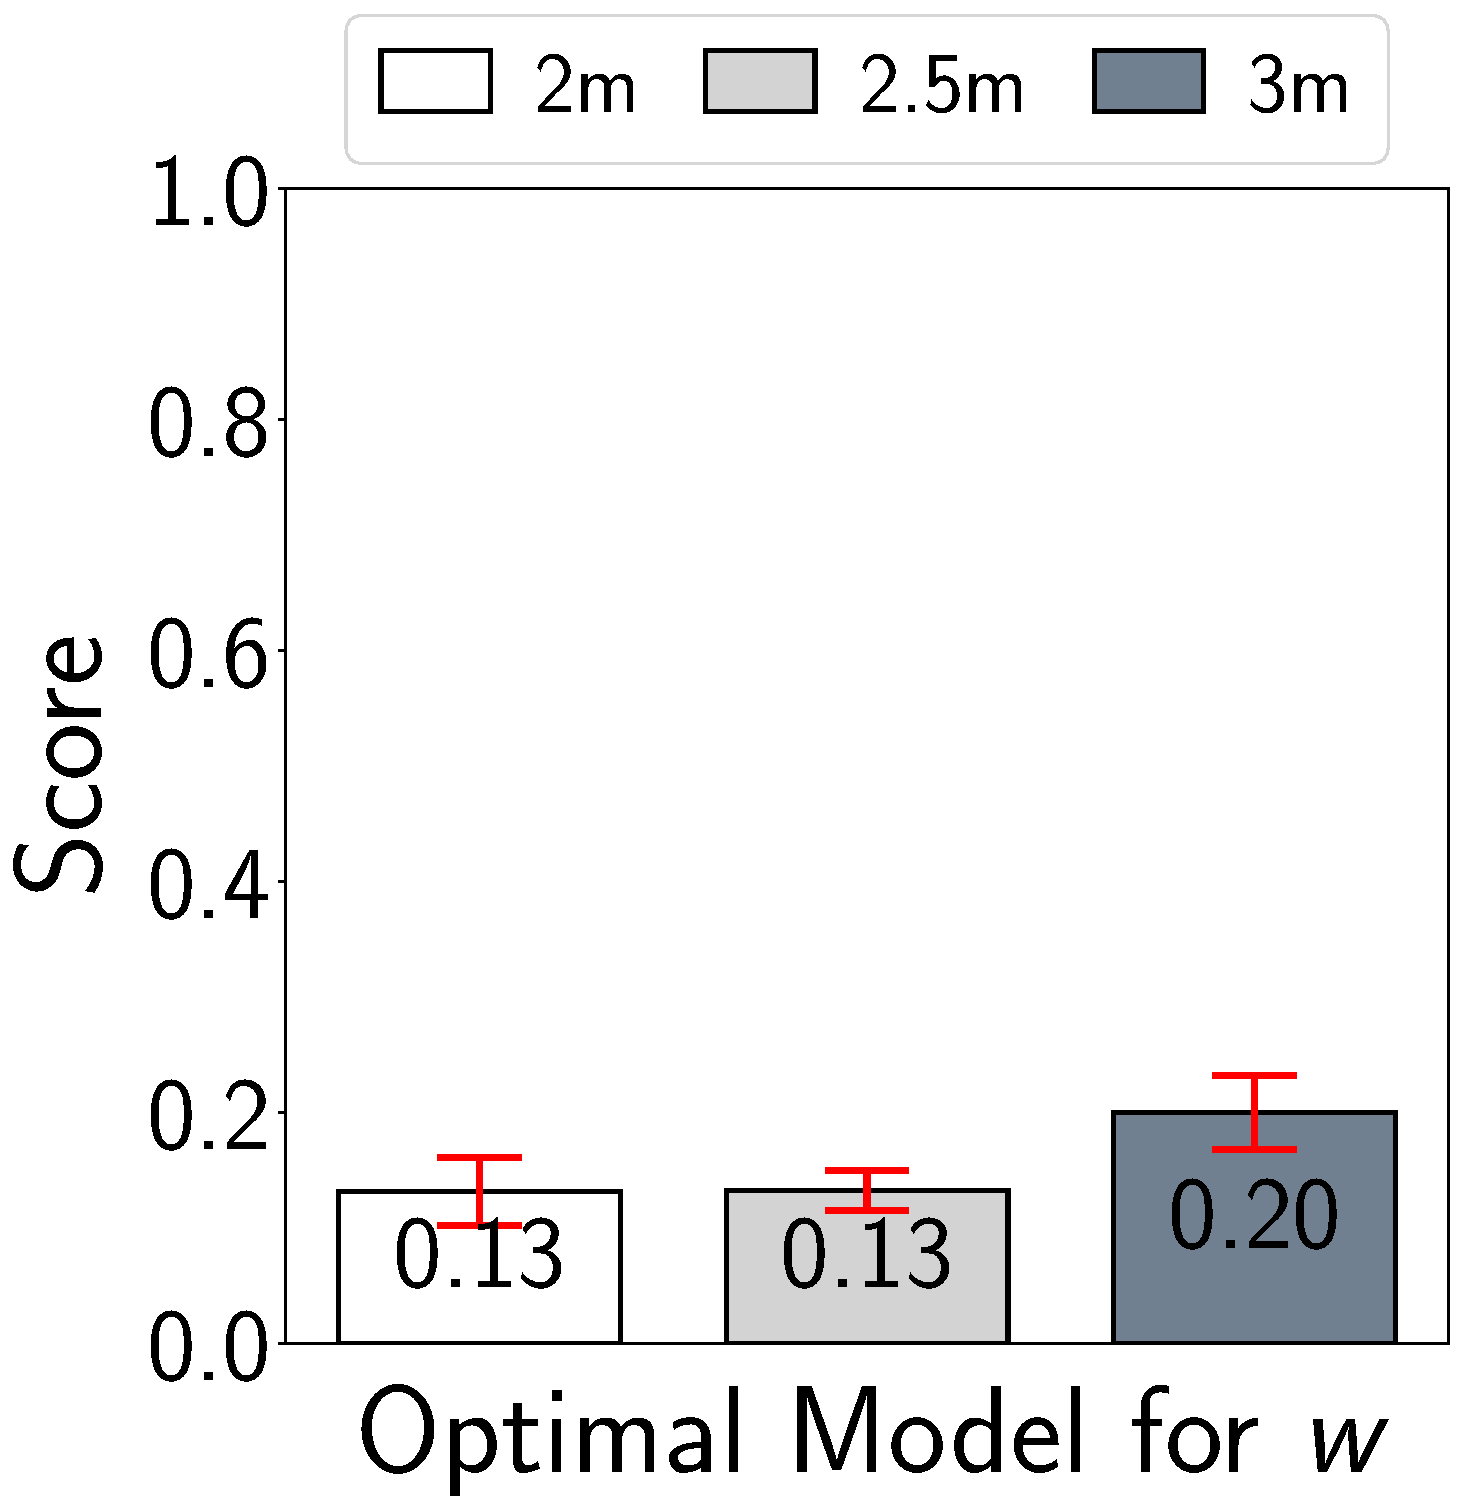
\includegraphics[width=1.0\linewidth]{chapter6/FIGS/fig-avoidance-best.pdf}\\
\caption{Baseline Scores}
\label{fig:avoid-best}
\end{minipage}
\begin{minipage}{0.45\linewidth}
\centering
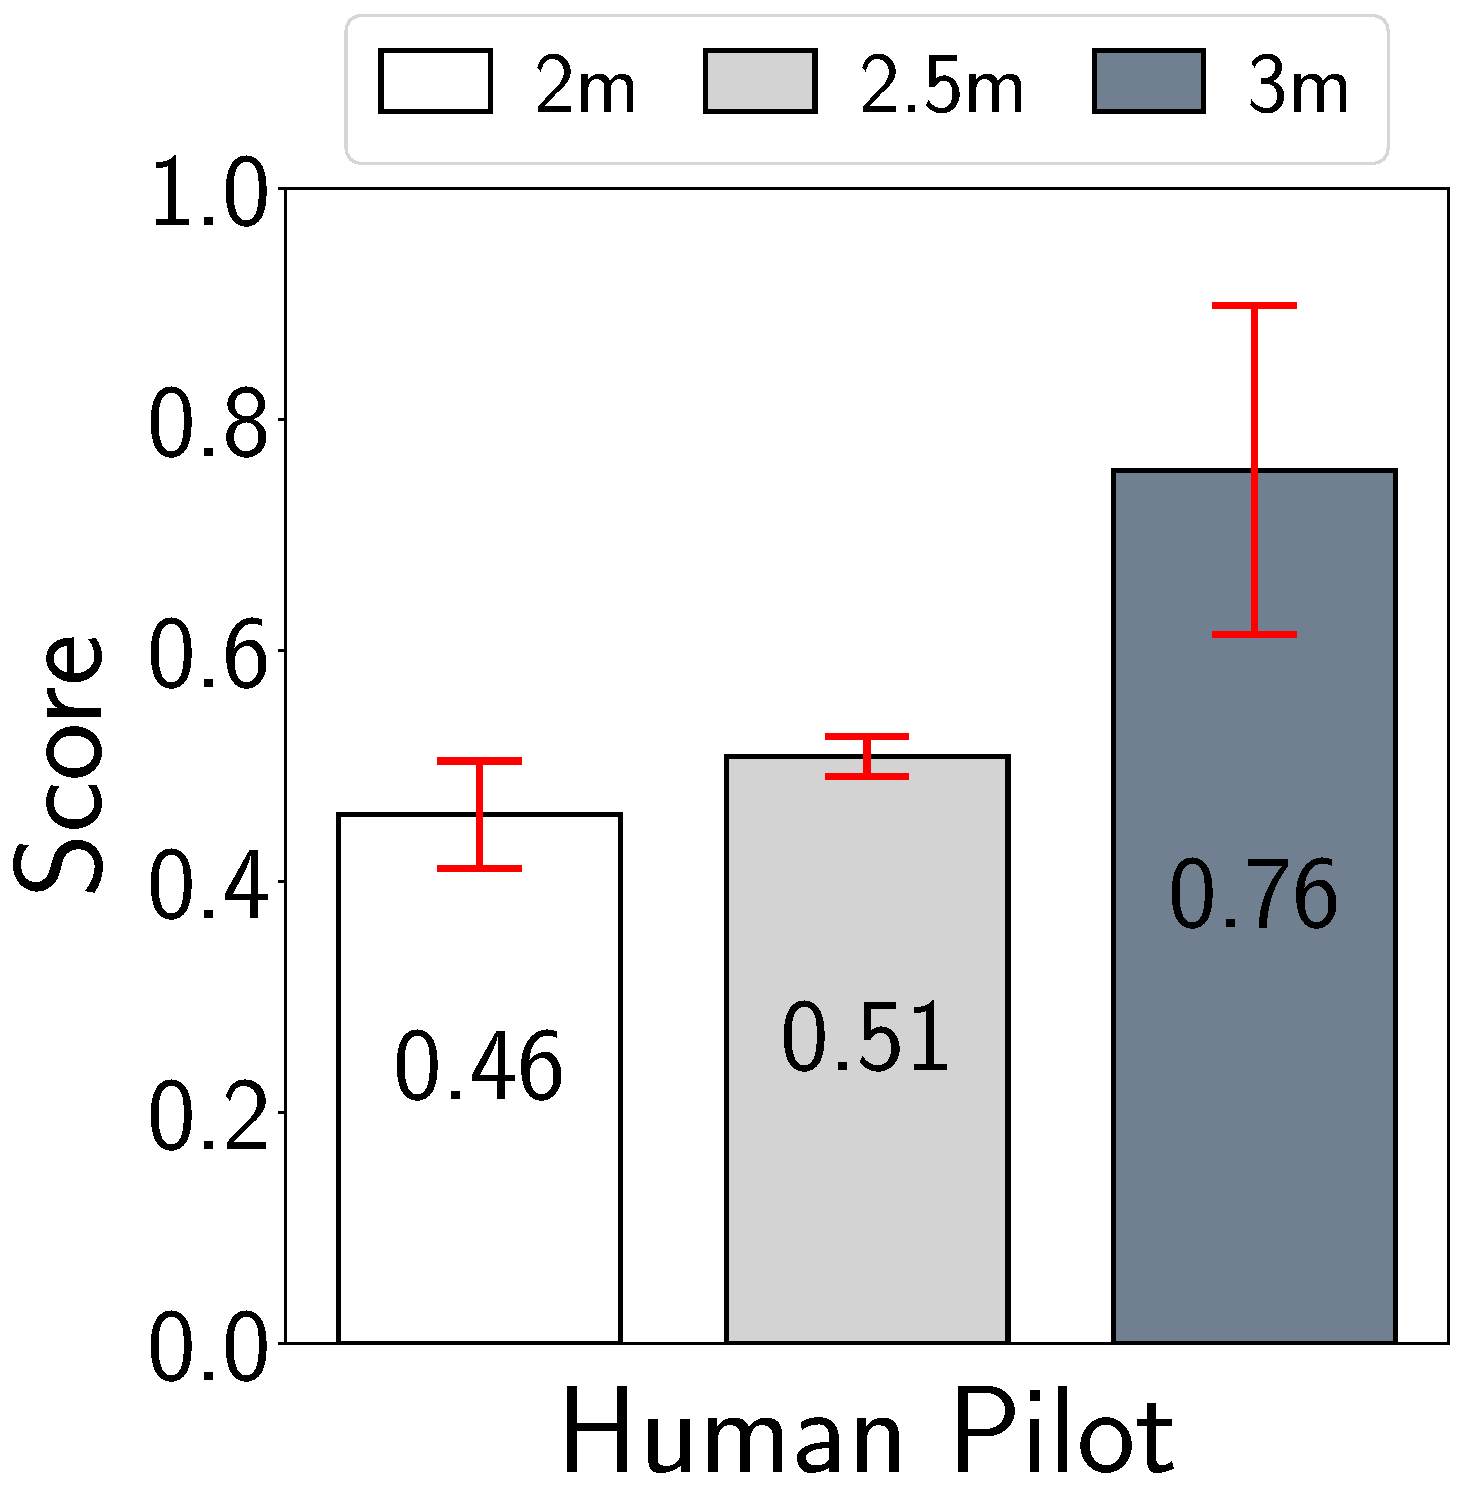
\includegraphics[width=1.0\linewidth]{chapter6/FIGS/fig-avoidance-human.pdf}\\
\caption{Human Pilot}
\label{fig:avoid-human}
\end{minipage}
\end{figure}


\begin{figure}
\centering
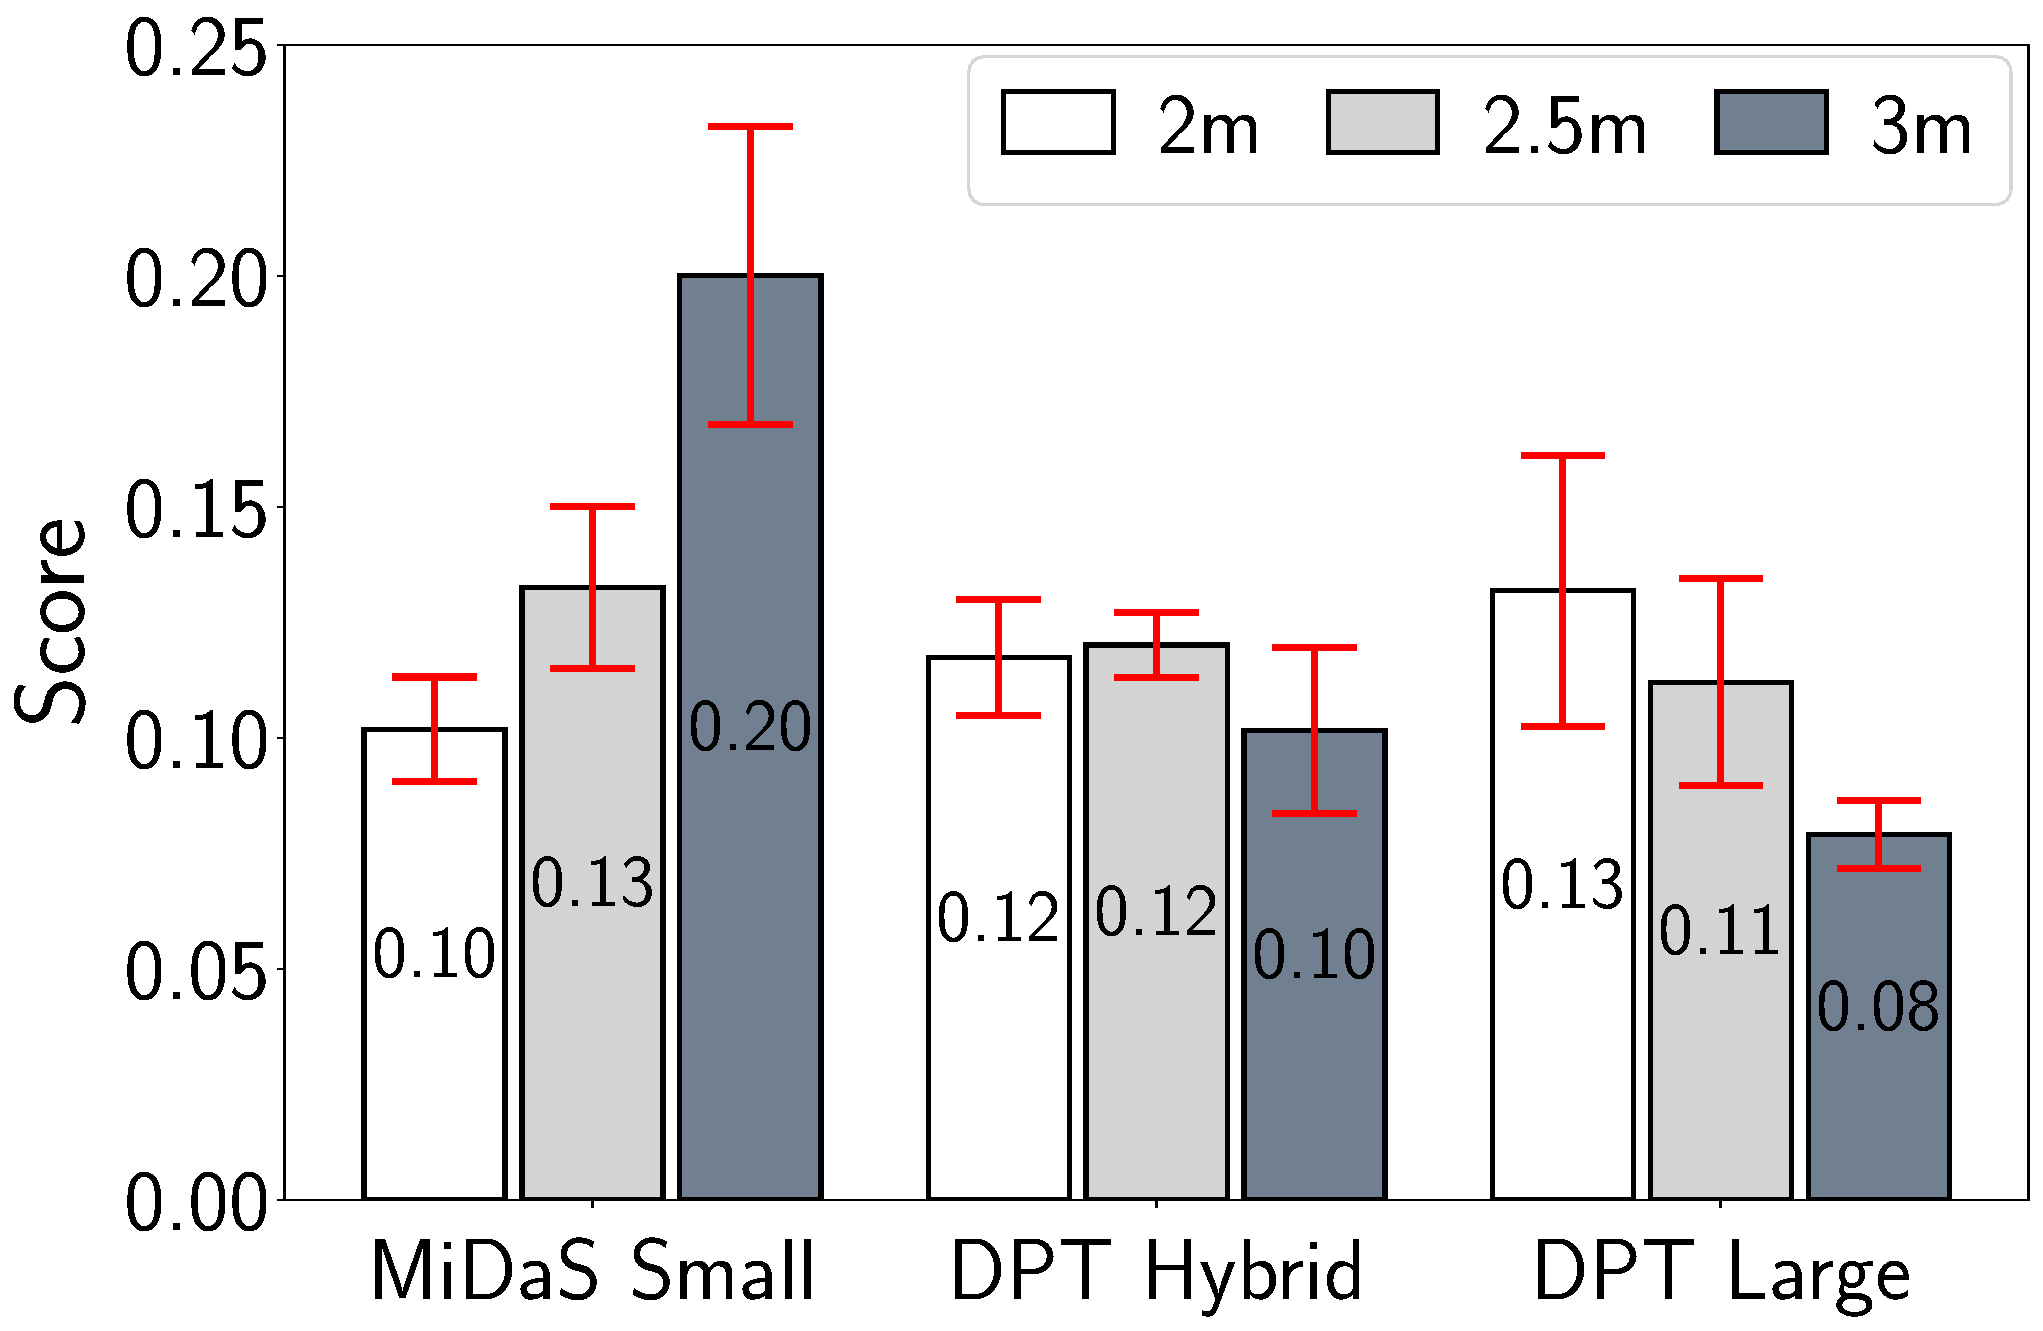
\includegraphics[width=0.8\linewidth]{chapter6/FIGS/fig-avoidance-models.pdf}
\caption{Impact of MiDaS Model on Avoidance Benchmark}
\label{fig:avoidance_by_model}
\end{figure}


\subsection{Impact of Model Accuracy}
\label{sec:avoidance-models}
The availability of the different MiDaS models shown in
Table~\ref{tab:midas-model-stats} leads to the question:
\begin{itemize}
\item{\em Is accuracy or speed  more important?}
\end{itemize}
My experiments indicate that there is no simple answer to this
question.  The results in Figure~\ref{fig:avoid-best} were
obtained using the best MiDaS model for each value of $w$.  MiDaS
Small performs the best on the 3~m course but worst on the 2~m course.
DPT Large is the inverse, performing best on the 2~m course and worst
on the 3~m course.  DPT Hybrid stays consistently in the middle for
all three courses.  The fact that different models had to be used in
each case to obtain the best results indicates that there is no single
``best'' model.  

I conducted a set of experiments to better understand this tradeoff
space.  The results in Figure~\ref{fig:avoidance_by_model} show the
score achieved on the benchmark for each model and value of $w$.
Since MiDaS Small focuses on throughput and low latency over accuracy,
a drone that uses it is able to sustain a higher maximum speed than
one using DPT Large.  At $w = $3~m, the course is sufficiently easy
that the increased risk of collision is small.  The higher accuracy of
a better model is not useful.  However, at $w = $2~m, the increased
likelihood of collisions makes higher model accuracy worthwhile.  Now,
DPT Large attains the highest score.  For a tight course, it is
difficult to travel at high speed without collisions. Hence, a model
that can navigate the gaps better gets a higher  score.

\begin{figure}
\centering
\begin{minipage}{0.8\linewidth}
\centering
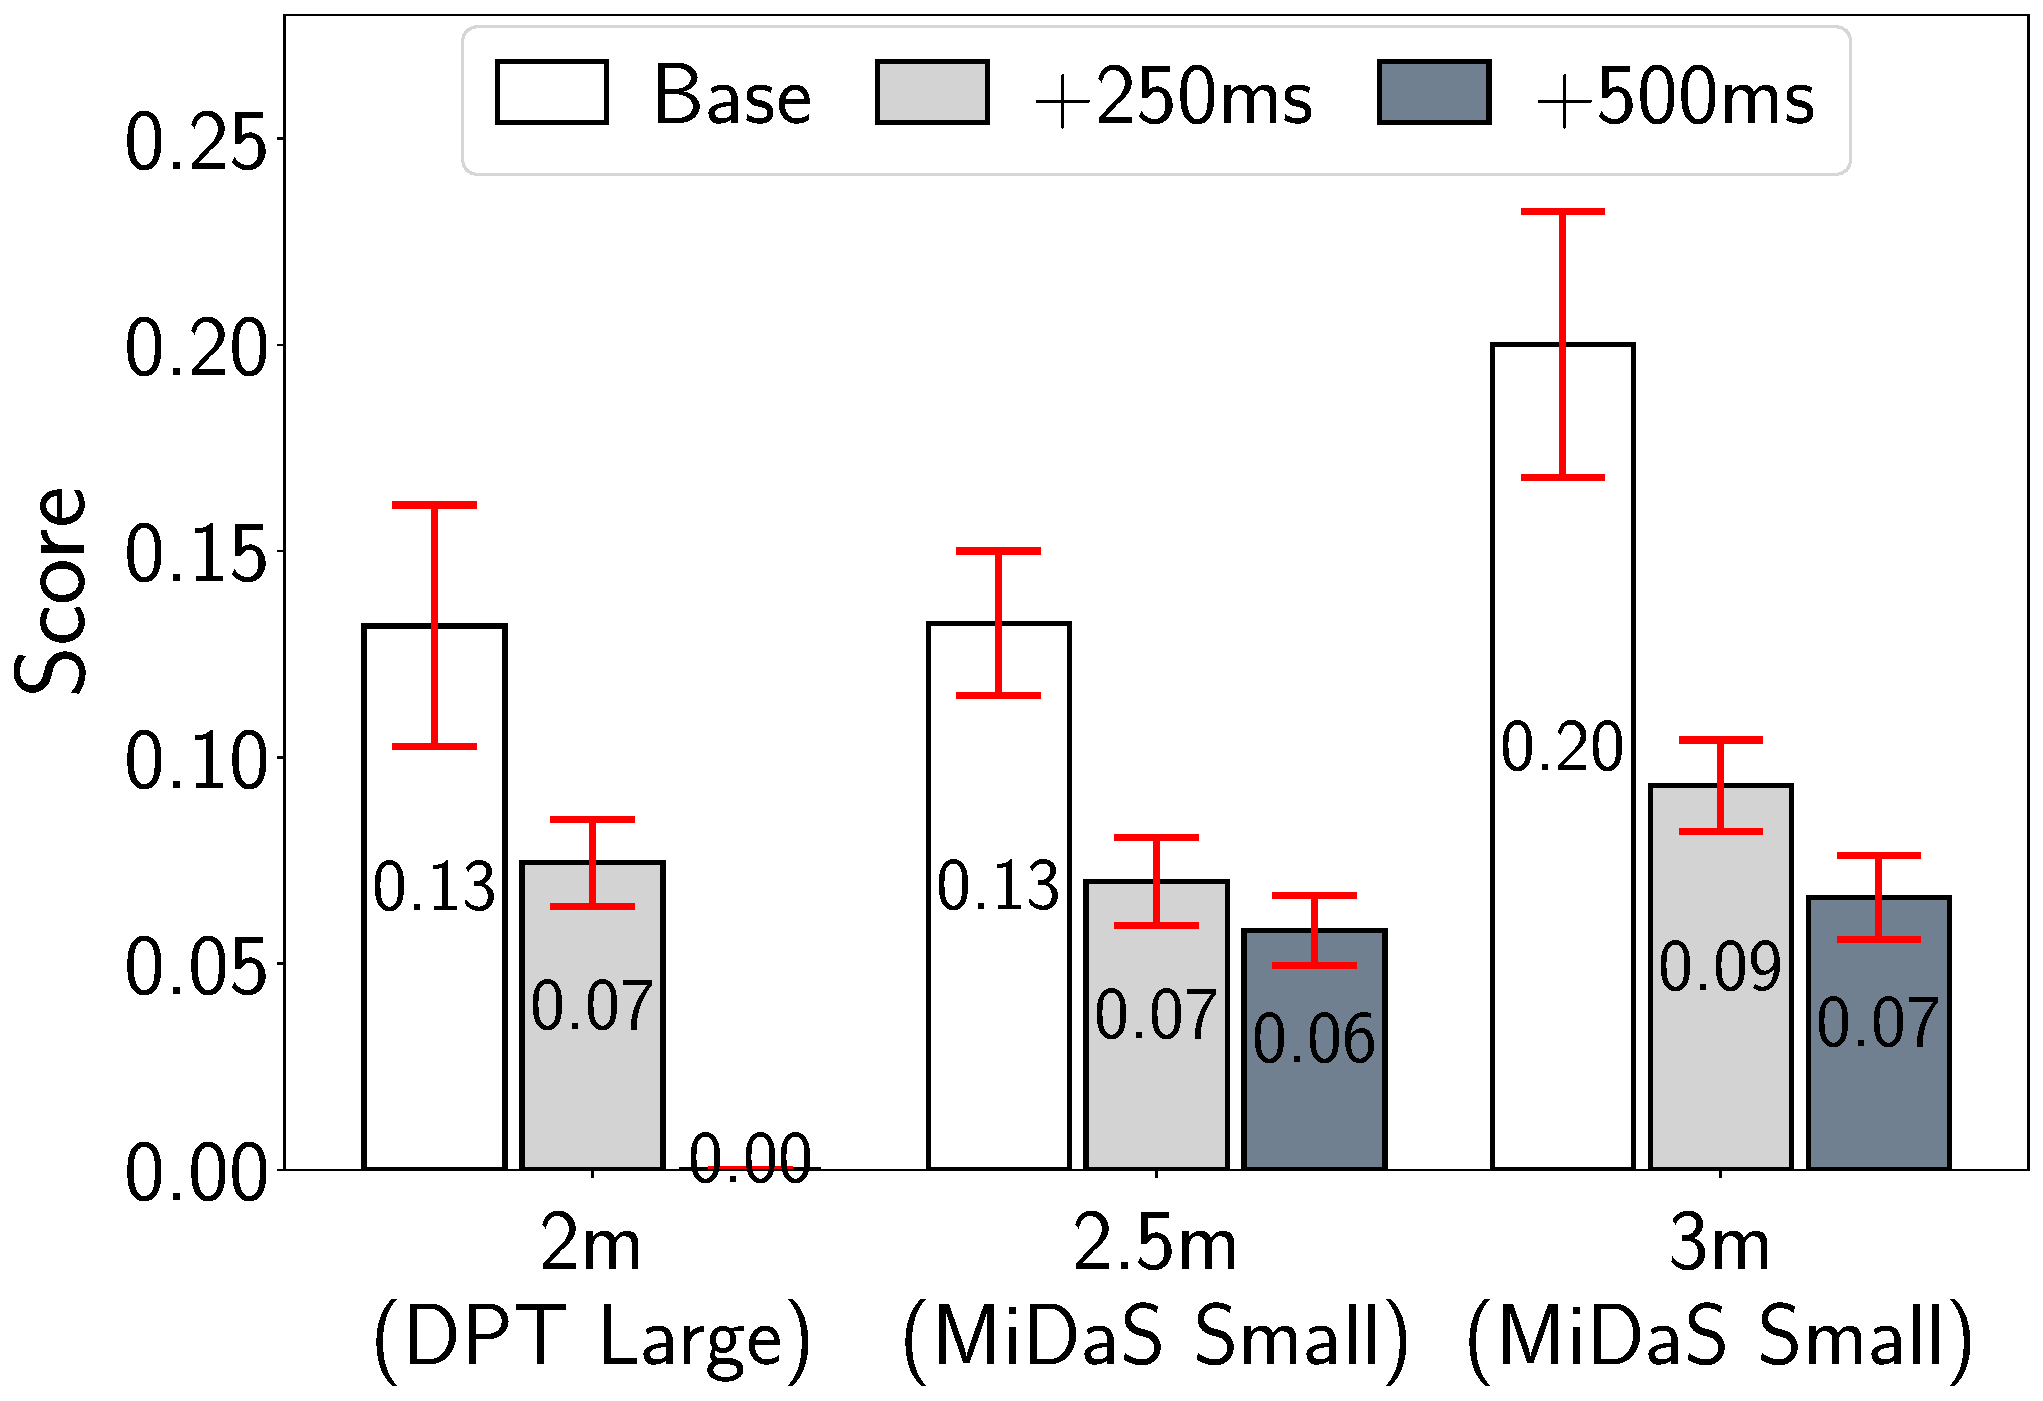
\includegraphics[width=0.96\linewidth]{chapter6/FIGS/fig-avoidance-latency.pdf}
(a) Additional Latency
\end{minipage}
\begin{minipage}{0.8\linewidth}
\centering
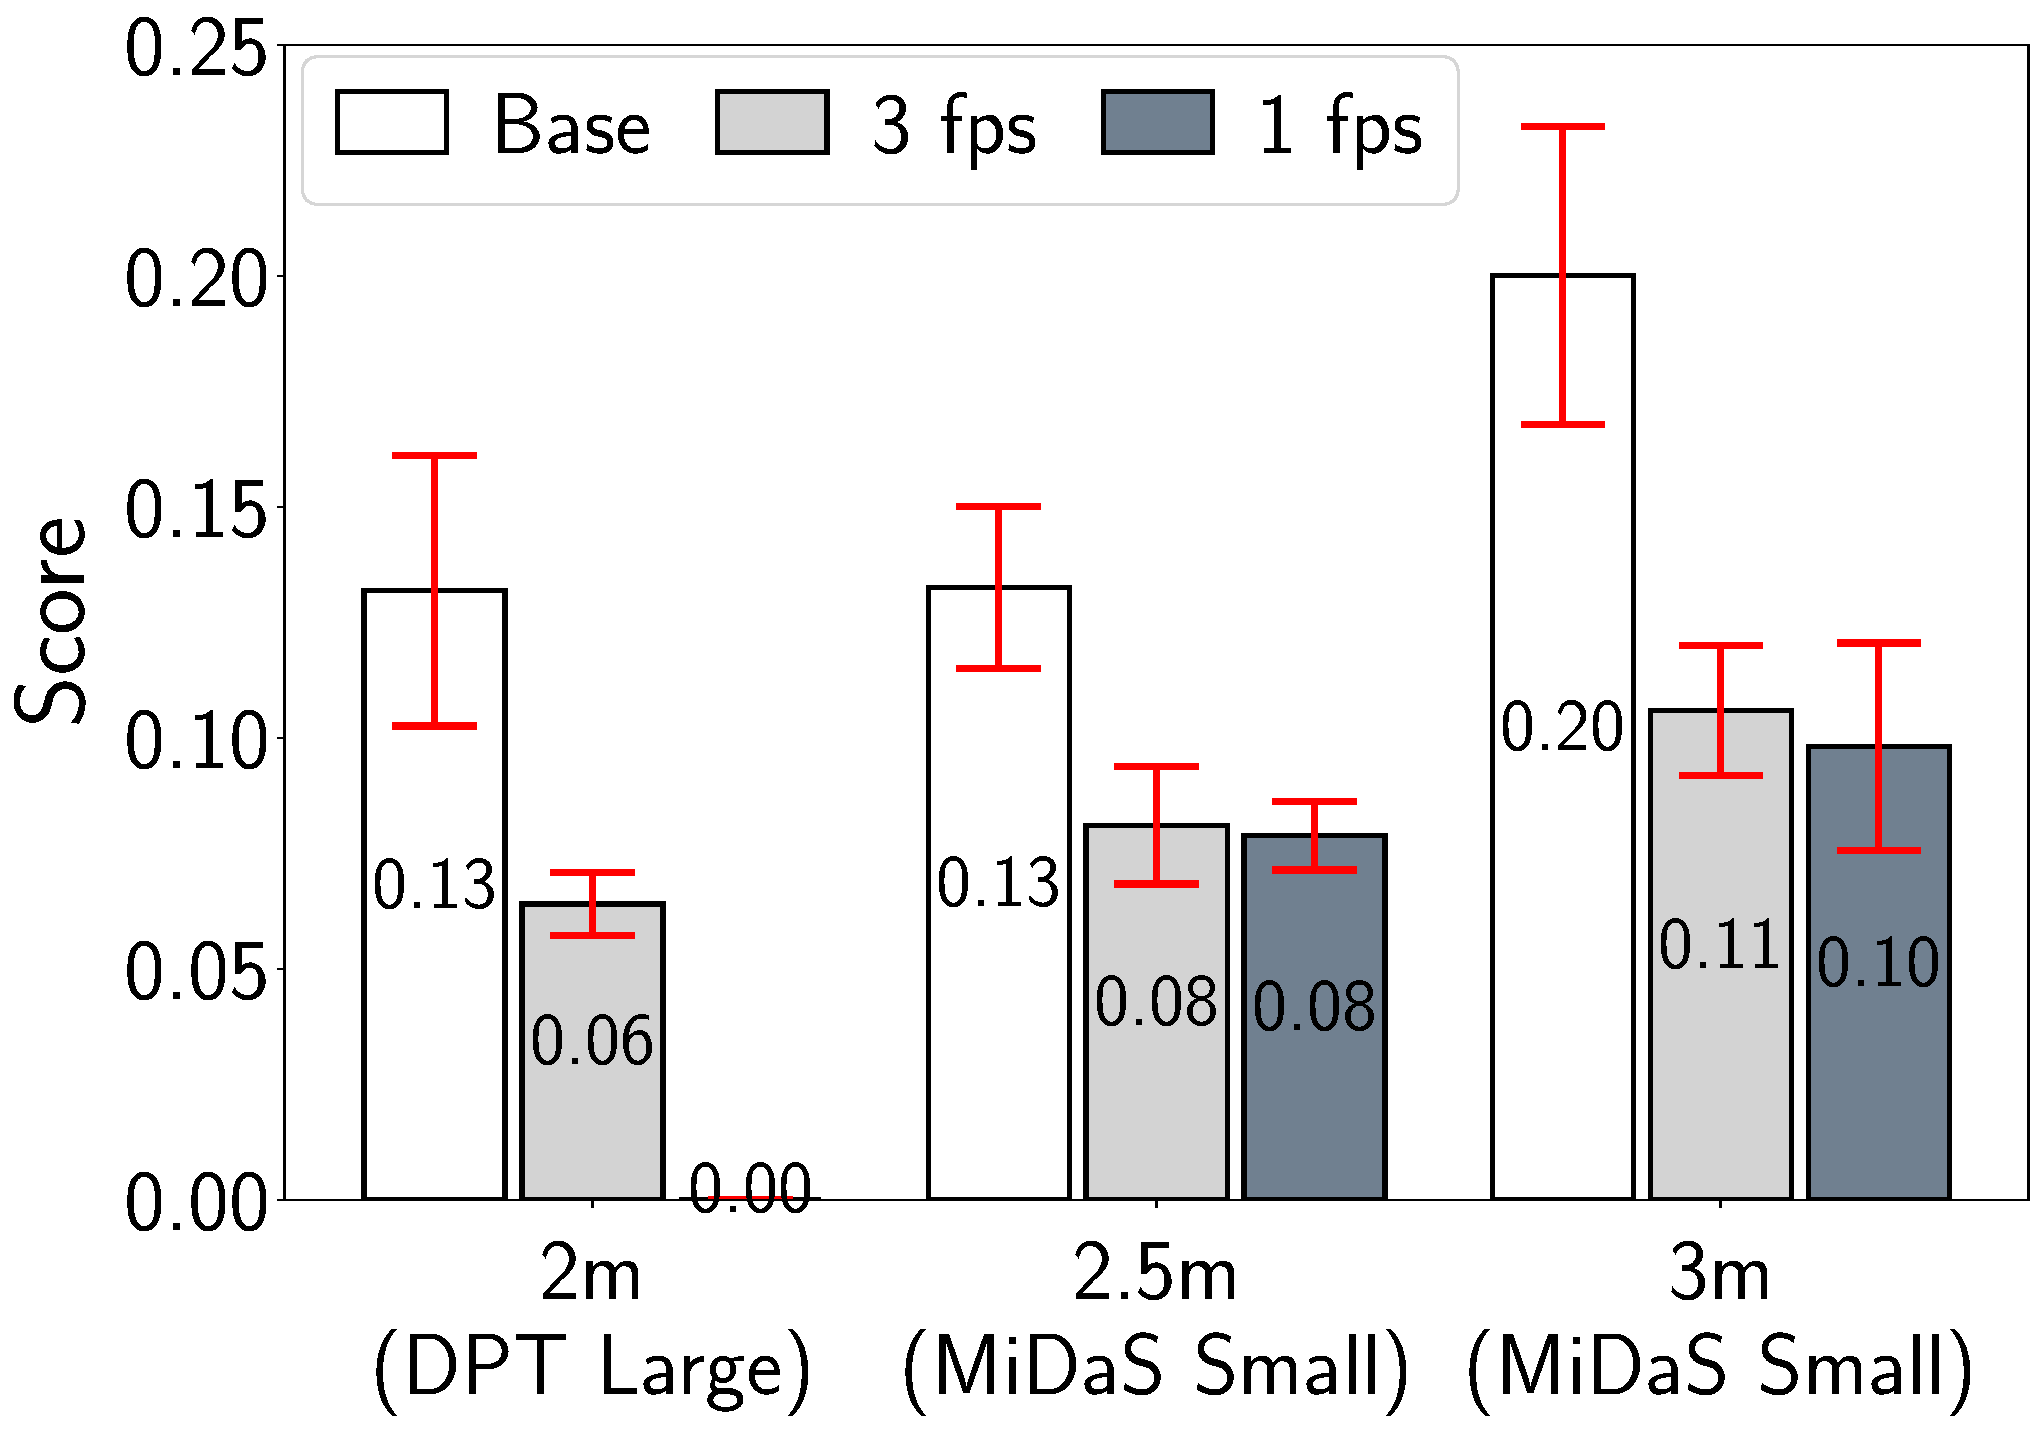
\includegraphics[width=0.96\linewidth]{chapter6/FIGS/fig-avoidance-fps.pdf}
(b) Reduced Throughput
\end{minipage}
\caption{Impact of Latency and Throughput on Avoidance}
\label{fig:avoidance-latency-throughput}
\end{figure}

\subsection{Impact of Latency \& Throughput}
\label{sec:avoidance-factors}

The results presented so far reflect best-case conditions.  In
practice, the wireless network or the cloudlet may suffer degradation
due to multi-tenancy.  This leads to the question:
\begin{itemize}
\item{\em What is the impact of latency or throughput degradation of
    the \ooda~loop on benchmark score?}
\end{itemize}
The baseline scores reflect what is
achievable with an \ooda~loop whose latency is the sum of three
components:
\begin{itemize}
\item{a lower bound of 527~ms~(Figure~\ref{fig:ooda-scaling}).}

\item{the latency of the relevant MiDaS model~(Table~\ref{tab:midas-model-stats}).}

\item{a small additional overhead ($<$1~ms) for Stage-3 processing
    in the Decide part of the \ooda~loop.}
\end{itemize}

This total end-to-end latency is on the order of 600--650~ms.  For
\ooda~loop iterations that involve drone actuation, the bottleneck
throughput is the smaller of 6~fps for
Act$_{fg}$~(\S\ref{sec:c2d-drone}) and the throughput of the MiDaS
model~(Table~\ref{tab:midas-model-stats}).  This is effectively
6~fps, regardless of model.  If no drone actuation is involved, the
bottleneck throughput becomes that of the MiDaS model.  Since even
MiDaS Small has lower throughput than Observe$_{ab}$, Observe$_{c}$,
or best-case Orient+Decide$_d$, throughput is always in the 6--10~fps
range.

Figure~\ref{fig:avoidance-latency-throughput}(a) shows how benchmark
score drops as latency is artificially added to the \ooda \\ loop.  Even
250~ms of additional latency (i.e., a roughly 35--40\% increase from
baseline) causes benchmark score to drop to nearly half its baseline
value, for all values of $w$ and regardless of MiDaS model.  If 500~ms
of latency is added, the score drops further.  For the most
challenging course~($w = 2$~m), the score drops to zero because not
even 80\% of the flights are successful.  These results are consistent
with a long-standing design principle of deeply-immersive closed-loop
interactive systems: {\em increased latency is deadly, even if
  throughput remains good.}

Figure~\ref{fig:avoidance-latency-throughput}(b) shows how benchmark
score drops as the throughput of the \ooda~loop is artificially
reduced from its baseline value.  Reducing throughput to 3~fps causes
benchmark score to drop to nearly 40--50\% of its baseline value.  A
further drop is observed when throughput is reduced to 1~fps.  For $w
= 2$~m, the benchmark score drops to zero.  These results confirm that
latency is not the sole determinant of task performance in an
\ooda~loop --- throughput also matters.

\subsection{Value of On-board Drone Intelligence}
\label{sec:djiminipro}

Edge computing allows use of compute resources that are far larger and heavier than could be carried by an ultralight drone.  In the context of AI,
this translates to {\em generality} and {\em versatility}.  Purely
through software development on the cloudlet, it is easy to re-purpose
the drone for new tasks that were not anticipated earlier.

\begin{figure}
\small
\centering
\begin{tabular}{lr}
  \hline
  Architecture & Efficiency (GFLOP / J) \\
  \hline
  CPU (Core i7)        & \phantom{0}1.14  \\
  FPGA (Xilinx LX760)  & \phantom{0}3.62  \\
  GPU (NVIDIA GTX285)  & \phantom{0}6.78  \\
  GPU (AMD R5870)      & \phantom{0}9.87  \\
  ASIC                 & 50.73 \\
  \hline
\end{tabular}
\begin{captext}
\\[0.2cm] \small Source: Table 4 in Chung et al~\cite{Chung2010}
\end{captext}
\caption{Matrix Multiplication Kernel Implementations}
\label{fig:energy2}
\end{figure}

The drone marketplace, however, is moving in the opposite direction.
Drone vendors are constantly identifying specific new functionality to
add to drones. There is a well-understood tradeoff between
generality, energy-efficiency, development cost, and weight/size that
applies in this context. As Figure~\ref{fig:energy2} from Chung et
al~\cite{Chung2010} shows, an ASIC is by far the most energy efficient
alternative for a given functionality.  It is also likely to have the
lowest weight.  But, it takes much longer to develop, is much more
expensive to create than pure software, and only provides fixed
functionality.

To quantify the value of on-board intelligence, I re-ran my obstacle
avoidance benchmark using a DJI Mini 4 Pro drone, seen in Figure~\ref{fig:drone-anatomy}.  This consumer
photography drone weighs 249~g, and is equipped with 6 stereo cameras
and an onboard obstacle avoidance system. It has two modes, Normal and
Nifty. Normal prioritizes safe flight while Nifty attempts to pass
obstacles as quickly as possible.  The obstacle avoidance feature of
this drone is intended as a form of ``pilot assist.''  The RPIC flies
the drone without worrying about obstacles.  The drone's builtin
capability performs all the necessary sensing and actuation needed to
avoid collisions.

Figure~\ref{fig:avoidance_dji} presents the scores obtained by the DJI
Mini 4 Pro  on my obstacle avoidance benchmark.  The baseline results
for my platform from Figure~\ref{fig:avoid-best} are also shown for
comparison.  For all values of $w$, the DJI Mini 4 Pro  is at a clear
advantage.  This the direct result of additional sensors and a much
faster \ooda~loop that avoids edge offload.

\begin{figure}
\centering
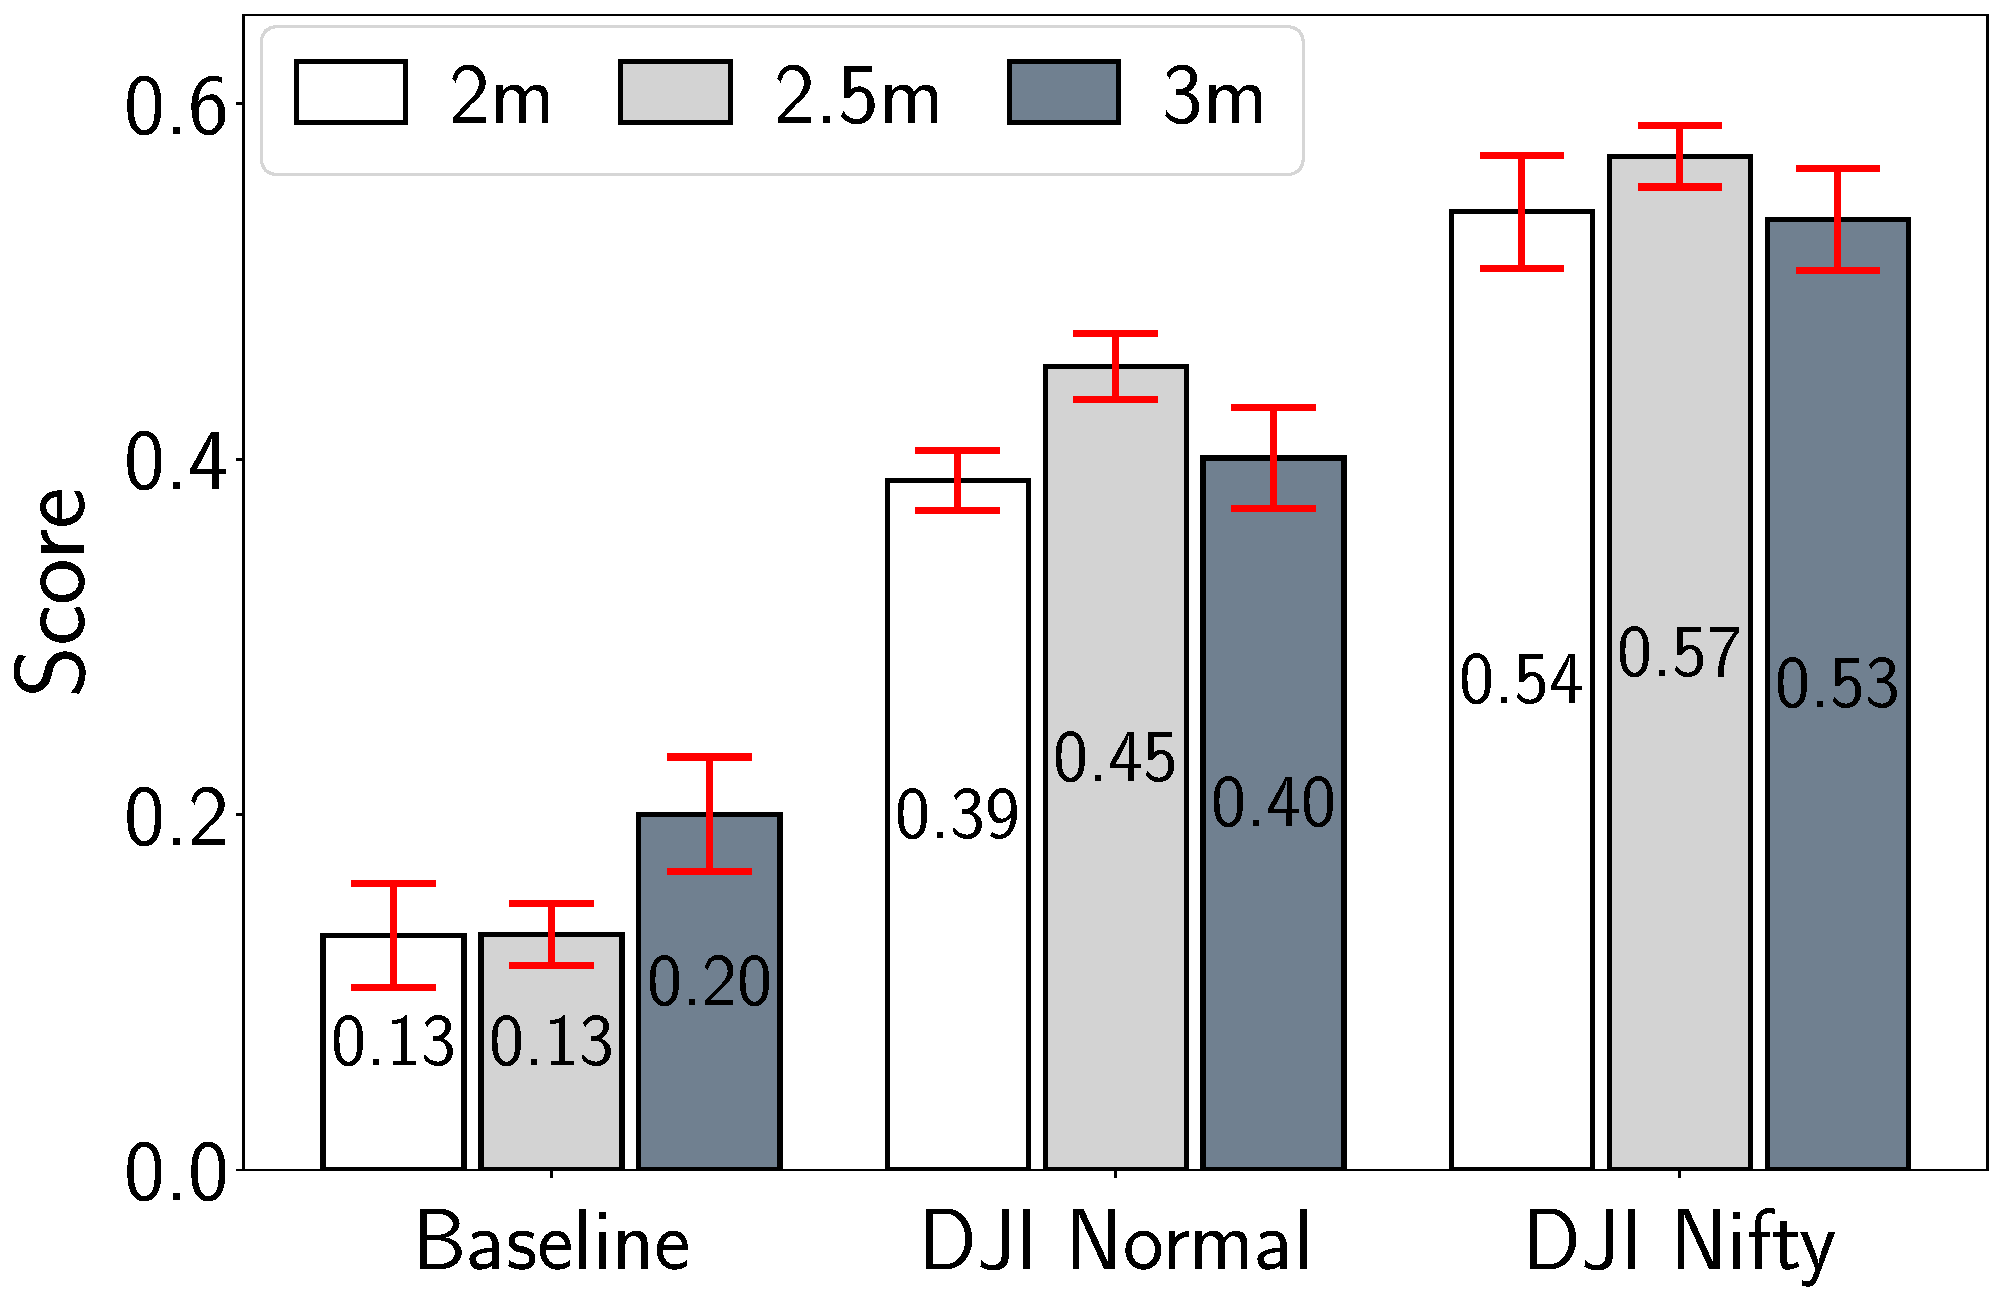
\includegraphics[width=0.8\linewidth]{chapter6/FIGS/fig-avoidance-dji.pdf}
\caption{On-Board Obstacle Avoidance}
\label{fig:avoidance_dji}
\end{figure}

These results suggest that even when using edge offload, there is very
clear value in taking advantage of on-board capabilities when they are
available.  The ``pilot assist'' approach to obstacle avoidance
implemented by the DJI Mini 4 Pro could equally well be used by
cloudlet-based software to control the drone's flight path.  Only the
macro components of that flight path would incur the overhead of the
\ooda~loop from drone to cloudlet.  The micro components of the flight
path that maneuver the drone around obstacles would only be subject to
its much tighter on-board \ooda~loop.

Complementing on-board fixed functionality with edge offload provides
extensibility and versatility.  The DJI Mini 4 Pro, for example, is
unable to do general-purpose object detection even though it can
detect people and vehicles.  It cannot detect the Robomaster target, and is hence
unable to execute my tracking benchmark.  Edge offload could remedy
that limitation, thereby increasing the versatility of the drone.